\documentclass{article}
\usepackage[style=apa, backend=biber]{biblatex}
\addbibresource{hopping.bib}
\usepackage{graphicx}
\usepackage{booktabs}
\usepackage{indentfirst}
\usepackage{amsmath}
\usepackage{setspace}
\usepackage[margin=1in]{geometry}
\usepackage[table,x11names]{xcolor}
\usepackage{fancyhdr}
\usepackage{tabularx}
\usepackage[compact]{titlesec}
\usepackage{listings}
\usepackage{color}
\usepackage{fontspec}
\usepackage{unicode-math}
\pagestyle{fancy}
\fancyhf{}
\renewcommand{\headrulewidth}{0pt}
\fancyhead[R]{\thepage}
\titleformat{\section}[block]{\normalsize\bfseries}{}{0em}{}
\titleformat{\subsection}[block]{\normalsize\bfseries}{}{0em}{\itshape}
\titleformat{\subsubsection}[block]{\normalsize}{}{0em}{\itshape}
\doublespacing
\setmainfont{DejaVu Serif}
\setmathfont{DejaVu Math TeX Gyre}
\setmonofont{DejaVu Sans Mono}
\definecolor{dkgreen}{rgb}{0,0.6,0}
\definecolor{gray}{rgb}{0.5,0.5,0.5}
\definecolor{mauve}{rgb}{0.58,0,0.82}

\lstset{frame=tb,
  language=C,
  aboveskip=3mm,
  belowskip=3mm,
  showstringspaces=false,
  columns=flexible,
  basicstyle={\small\ttfamily},
  numbers=none,
  numberstyle=\tiny\color{gray},
  keywordstyle=\color{blue},
  commentstyle=\color{dkgreen},
  stringstyle=\color{mauve},
  breaklines=true,
  breakatwhitespace=true,
  tabsize=3
}

\begin{document}
\begin{titlepage}
	\centering
	\vspace*{0.2\textheight}
	\textbf{}\\
	Lyndsay Ricks\\
	Department of Biology, University of Utah\\
	BIOL 3665: Animal Form and Function\\
	Colleen Farmer\\
	April 14, 2023
\end{titlepage}
\section{Abstract}

{\parindent0pt abstract abstract abstract} \\

{\parindent0pt Keywords: \emph{cardiorespiratory fitness, VO$_2$max, physiology, human biology, support vector machines}}

\pagebreak

\section{Introduction}

\section{Materials and methods}
\subsection{Participants}
Participants were drawn from a pool of nine undergraduate students enrolled in a biological form and function laboratory course at the University of Utah (Salt Lake City, UT, USA), of whom eight, including the author, ultimately provided all requisite data. Of the participants, five were female and three were male. Apart from age, the demographic and health information provided by participants varied quite widely, as is summarized in Table \ref{fig:summary}, providing a reasonably accurate approximation of the overall population. 
\begin{table}[h!]
\centering
\begin{tabularx}{\linewidth}{Xllll}
\toprule
Variable                                        & Median & Mean  & Standard deviation & Range (min-max) \\ \midrule
Age (years)                                     & 22     & 22.6  & 3.1                & 18-27           \\
Weight (kg)                                     & 66.8   & 70.5  & 13.5               & 58-99           \\
Height (m)                                      & 1.71   & 1.72  & 0.076              & 1.64-1.87       \\
Resting heart rate (bpm)                        & 73.5   & 73.3  & 10.6               & 60-88.5         \\
Heart rate after 20 min moderate exercise (bpm) & 116    & 120.5 & 23.3               & 89-153          \\
Heart rate after 10 min vigorous exercise (bpm) & 135    & 143.5 & 25.0               & 118-182         \\
Sum of answers to PFA questionnaire             & 14.5   & 13.9  & 4.3                & 6-21            \\
Frequency I (calculated via computer)                      & 0.76   & 0.82  & 0.48               & 0.29-1.56       \\
Frequency II (counted manually)                        & 0.73   & 0.80  & 0.44               & 0.33-1.55       \\ \bottomrule
\end{tabularx}
	\caption{Summary statistics for participant demographics ($n = 8$).}
	\label{fig:summary}
\end{table}

\subsection{Data gathering}
Owing to time and budget constraints, not all of the potential predictors of VO$_2$max identified and tested by \textcite{abut2016} could be measured. The various maximal and submaximal metrics they selected were collapsed into a simple measurement of heart rate after 10 minutes of vigorous and 20 minutes of moderate aerobic exercise (selected by the participant). Basic demographic variables were retained, as well as the PFA questionnaire (see Supplementary Material), which was identified as a relatively strong discriminator. The PAR questionnaire was not given to participants, as \textcite{abut2016} found it to be much weaker than the PFA questionnaire. Participants were instructed to obtain their resting heart rate by measuring at four times and calculating the average.

Participants' preferred hopping frequencies were simultaneously measured in two different ways — digitally and manually. For the digital portion, participants utilized Blackboard microcontroller boards and three-dimensional QWIIC accelerometers (both from SparkFun Electronics, Niwot, CO, USA). Participants affixed both the microcontroller board and the attached accelerometer to a chosen stable portion of their body and used the official Arduino IDE (Arduino, Turin, Italy) to execute a script (see Supplementary Material) to obtain acceleration values on all axes at short intervals as they hopped up and down regularly at a pace comfortable to them for a total of 120 seconds. Participants identified crests in the resulting waveform and reported frequencies obtained from the average distance from each crest to the next; this value is hereafter referred to as frequency I. Participants also manually counted how many times they jumped in the same session and divided this count by the length of time in order to obtain a separate measurement of frequency, which is referred to here as frequency II. For the most part, frequencies I and II were very similar, but not identical, within participants' estimates.

All information in the dataset used was self-reported by participants and measured in uncontrolled and potentially unstandardized environments; although participants were given clear general instructions as to how to measure each variable (included in Supplementary Material), specifics were left to their discretion.
\begin{figure}[h!]
	\centering
	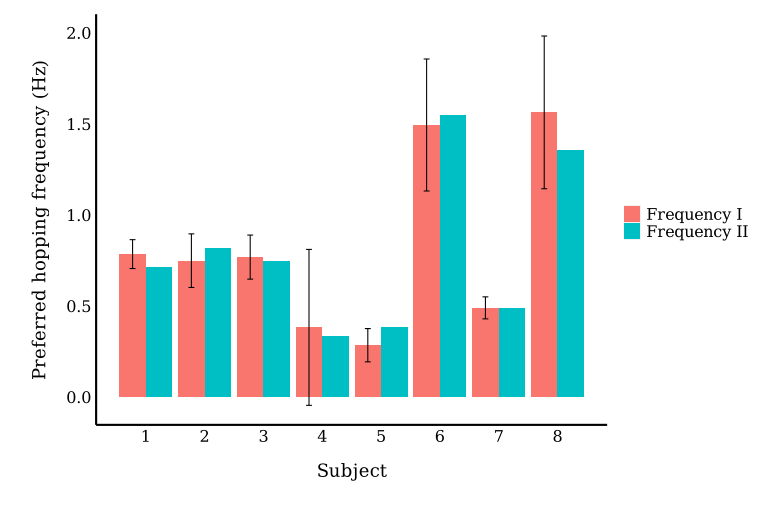
\includegraphics[width=0.75\linewidth]{plots/preference.png}
	\caption{Distribution of hopping frequencies among participants (error bars: $\bar x \pm \sigma$).}
	\label{fig:freqplot}
\end{figure}

\subsection{Analysis}
Analysis was conducted in R version 4.2.2 \parencite{r} using the packages \texttt{FSinR} \parencite{fsinr} for feature selection; \texttt{data.table} \parencite{datatable}, \texttt{dplyr} \parencite{dplyr}, and \texttt{tidyr} \parencite{tidyr} for data manipulation; \texttt{car} \parencite{car} for analyses of variance; and \texttt{ggplot2} \parencite{ggplot2} for production of graphics. Relevant features were identified using Relief-F scores at a threshold $\bar F > 0$ (across both frequency counts), selected by visual inspection \parencite{kira1992}. Considering the small sample size and the fact that only three predictors met the Relief-F threshold, it became clear that an SVM-based approach to categorizing the remaining predictors (as was taken by \cite{abut2016}) would be infelicitous; instead, I performed simple type II analyses of variance (assuming no interactions) modeling either frequency measurement as dependent on the predictors remaining after feature selection.

\section{Results}

\begin{table}[h!]
\centering
	\begin{tabularx}{\linewidth}{@{}XllX@{}}
	\toprule
	Predictor                          & Relief-F score (frequency I) & Relief-F score (frequency II) & Outcome                        \\ \midrule
	Age                                & $-0.050295218$                                       & $-0.062225137$                             & Excluded \\
	Sex                                & $0.040612306$                                        & $0.061634546$                              & Retained                       \\
	Weight                             & $0.115953009$                                        & $0.081889255$                              & Retained                       \\
	Height                             & $0.214929358$                                        & $0.254722111$                              & Retained                       \\
	Resting heart rate                 & $-0.064587039$                                       & $-0.067885327$                             & Excluded \\
	Heart rate after moderate exercise & $-0.047876574$                                       & $-0.047648223$                             & Excluded \\
	Heart rate after vigorous exercise & $0.007974116$                                        & $-0.006987602$                             & Excluded \\
	PFA questionnaire                  & $-0.003871271$                                       & $-0.020412946$                             & Excluded \\ 	\bottomrule
	\end{tabularx}
	\caption{Feature selection results.}
	\label{fig:relief}
\end{table}

Only sex, weight, and height exhibited strong enough Relief-F scores to be included in further analysis (Table \ref{fig:relief}). Relief-F scores were mostly similar regardless of which frequency measurement was used as the response variable, but the disparity was generally larger for the three positive predictors. Height exhibited the highest score by far for both frequency measurements.

\begin{table}[h!]
\centering
\begin{tabular}{@{}lllll@{}}
\toprule
Predictor & $F$-statistic (frequency I) & $p$-value (frequency I) & $F$-statistic (frequency II) & $p$-value (frequency II) \\ \midrule
Height    & 7.80                                   & 0.049 **                                 & 7.64                   & 0.051 *                  \\
Weight    & 1.77                                   & 0.25                                     & 0.58                   & 0.49                     \\
Sex       & 0.92                                   & 0.39                                     & 0.58                   & 0.49                     \\ \bottomrule
\end{tabular}
	\caption{Results of type II ANOVAs (*marginally significant, $p < 0.1$; **significant, $p < 0.05$).}
	\label{fig:anovas}
\end{table}

Type II analysis of variance revealed a marginally significant relationship between height and both frequency counts ($p \approx 0.05$), while no significant relationship was evident between weight or sex (which also had lower Relief-F scores) and hopping frequency (Table \ref{fig:anovas}).

\section{Discussion and conclusion}

The inherent limitations of this research design temper the extent to which any broader generalizations can be made. The fact that measurements were performed in an uncontrolled setting adds some amount of uncertainty to the accuracy of the raw data, and the small sample size relative to the wide variance of most variables means that robust individual points of comparison are lacking. 

\pagebreak
\printbibliography
\pagebreak
\section{Supplementary material}
\subsection{Instructions for data gathering}
No specific instructions were given for age, sex, weight, and height other than the units in which to provide them. For the other variables, instructions were as follows.
\subsubsection{Resting heart rate}
For the purposes of this analysis, please do your best to find a relaxing environment and spend at least 10-15 minutes there relaxing (preferably without distractions such as electronics) before taking a pulse. Make a tight fist and locate the pulse point of your radial artery just below your wrist on the thumb side of the large prominent tendon, as depicted below.

\begin{figure}[h!]
\centering
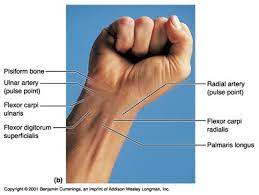
\includegraphics{pics/pulse.jpeg}
\end{figure}

Relax your fist and put pressure with two fingers at the pulse point until you feel a strong and clear pulse. Do NOT use your thumb to take a pulse, as it has its own pulse point and will complicate the results. After feeling 3 consecutive strong pulses, start a timer for 60 seconds or look at a clock for 60 seconds, counting the pulses throughout the whole minute. Record the number of pulses along with the date and time. Do this twice a day (once in the morning and once in the evening) for two consecutive days, recording the numbers each time. 

\begin{figure}[h!]
\centering
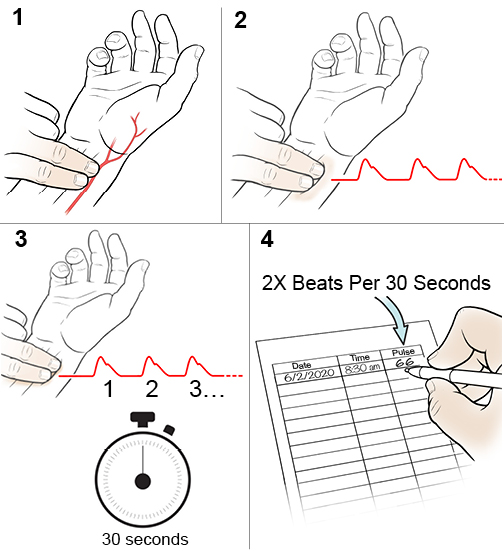
\includegraphics[width=0.6\linewidth]{pics/pulse2.jpeg}
\end{figure}

Average the four measurements you obtained.

\subsubsection{Heart rate with exercise}

Perform 20 minutes of aerobic exercise (jogging, cycling, swimming, etc.) that feels moderate (sustainable for that length of time, but somewhat challenging) and immediately afterwards, measure your heart rate one time the same way you did for your resting heart rate.

Perform 10 minutes of aerobic exercise (jogging, cycling, swimming, etc.) that feels intense/vigorous to you and immediately afterwards, measure your heart rate one time the same way you did for the other two measurements.

\subsubsection{PFA questionnaire}
The questionnaire is embedded below. Select a number between 1 and 13 that fits you for both questions and add the numbers that you chose together. Your result should be between 2 and 26. For example, if I think that jogging between a slow and medium pace is just right for me, and I could jog 3 miles at a pace between fast walking and slow jogging, I would answer 8+6 = 14.

\begin{figure}[h!]
\centering
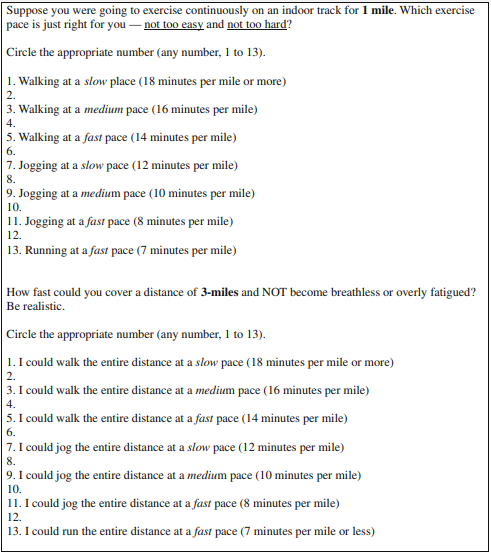
\includegraphics[width=0.8\linewidth]{pics/pfa.png}
\end{figure}

\subsection{Raw data and scripts}

\subsubsection{Arduino script}

The following script was used by participants to obtain their acceleration (provided by Mark Howell):

\begin{lstlisting}
#include <Wire.h>                 // Must include Wire library for I2C
#include "SparkFun_MMA8452Q.h"    // Click here to get the library: http://librarymanager/All#SparkFun_MMA8452Q
#include <math.h>

MMA8452Q accel;                   // create instance of the MMA8452 class

// Declare and initialize variables for acceleration readings
float xAccel = 0.;
float yAccel = 0.;
float zAccel = 0.;
float accelMag = 0.;
float correctionFactor = 2.0; // Needed for scales other than 2G, use 2 for 4G and 4 for 8G
long currentTime = 0L;
long checkTime = 0L;
int delayTime = 0;


// Sample rate, in Hz
float sampleRate = [selected by participant; >10];

void setup() {
    Serial.begin(115200);
    Wire.begin();
    if (accel.begin() == false) {
        Serial.println("Not Connected. Please check connections and read the hookup guide.");
        while (1);
    }
    //Adjust sensitivity to +- 4G, should prevent saturation
    accel.setScale(SCALE_4G);
    delayTime = 1000/sampleRate;
}

void loop() {
    while (Serial.available() == 0) 
    {
        if (accel.available()) {      // Wait for new data from accelerometer
            currentTime = millis();
            // Acceleration of x, y, and z directions in g units
            xAccel = accel.getCalculatedX() * correctionFactor;
            yAccel = accel.getCalculatedY() * correctionFactor;
            zAccel = accel.getCalculatedZ() * correctionFactor; 
            // Determine magnitude of acceleration vector
            // Determine magnitude of acceleration vector
            accelMag = sqrt(xAccel*xAccel + yAccel*yAccel + zAccel*zAccel);
            //checkTime = currentTime + delayTime;
            Serial.print("x = ");
            Serial.print("\t");
            Serial.print(xAccel, 3);
            Serial.print("\t");
            Serial.print("y = ");
            Serial.print("\t");
            Serial.print(yAccel, 3);
            Serial.print("\t");
            Serial.print("z = ");
            Serial.print("\t");
            Serial.print(zAccel, 3);
            Serial.print("\t");
            Serial.print("Mag = ");
            Serial.print("\t");
            Serial.print(accelMag, 3);
            Serial.print("\t");
            Serial.print("time = ");
            Serial.print("\t");
            Serial.print(currentTime/1000.,3);
            Serial.println();
            while (millis() < (currentTime + delayTime))
            {
                // Wait until enough time has passed for the next sensor check
            }
        }
    }
}
\end{lstlisting}

\subsection{Statistical analysis and raw data}
The R script for all analyses conducted for this project, the raw (anonymized) data, and the source code for this document are accessible via GitHub at https://www.github.com/lyndsayricks/biol3665.
\end{document}
